\subsection{Activation Functions}
Hidden units usually use a different activation function than the output units as it is independent of the type of problem we are trying to solve.

What's important to note is that in the choice of activation function it is much more important to consider the derivative 
of the function rather than the function itself, as it is what will be used during the backpropagation process to update the weights of the network.

\paragraph{Sigmoid}
Maps the input to a value between 0 and 1, which can be interpreted as a probability. It is defined as:
\begin{figure}[H]
    \centering
    \begin{minipage}{0.45\textwidth}
    \[
    \sigma(x) = \frac{1}{1 + e^{-x}}
    \]
\end{minipage}
\hfill
\begin{minipage}{0.45\textwidth}
    \centering
    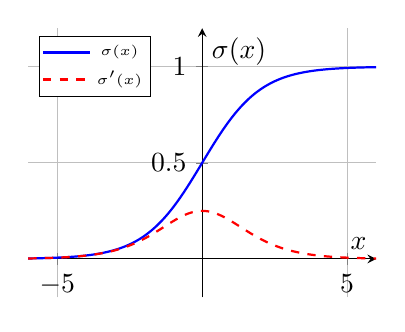
\begin{tikzpicture}[scale=1]
        \begin{axis}[
            xlabel=$x$,
            ylabel=$\sigma(x)$,
            grid=major,
            axis lines=middle,
            xmin=-6, xmax=6,
            ymin=-0.2, ymax=1.2,
            samples=200,
            width=6cm,
            height=5cm,
            legend pos=north west,
            legend style={font=\tiny, inner sep=1pt}
        ]
            \addplot[blue, thick, domain=-6:6] {1/(1+exp(-x))};
            \addlegendentry{$\sigma(x)$}
            \addplot[red, dashed, thick, domain=-6:6] {1/(1+exp(-x)) * (1 - 1/(1+exp(-x)))};
            \addlegendentry{$\sigma'(x)$}
        \end{axis}
    \end{tikzpicture}
\end{minipage}

\end{figure}
The function is smooth anddifferentiable everywhere, which is important for gradient-based optimization methods.
However, its derivative \textbf{saturate} (approaches 0) across most of its domain, which lead to the problem of vanishing gradients during training.

\paragraph{Hyperbolic Tangent (tanh)}
Similar to sigmoid but maps the input to a value between -1 and 1. It is defined as:
\begin{figure}[H]
    \centering
    \begin{minipage}{0.45\textwidth}
    \centering
    \[
    \tanh(x) = 2\sigma(2x) - 1 = \frac{e^x - e^{-x}}{e^x + e^{-x}}
    \]
\end{minipage}
\hfill
\begin{minipage}{0.45\textwidth}
    \centering
    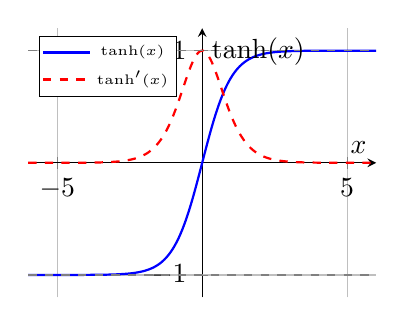
\begin{tikzpicture}[scale=1]
        \begin{axis}[
            xlabel=$x$,
            ylabel=$\tanh(x)$,
            grid=major,
            axis lines=middle,
            xmin=-6, xmax=6,
            ymin=-1.2, ymax=1.2,
            samples=200,
            width=6cm,
            height=5cm,
            legend pos=north west,
            legend style={font=\tiny, inner sep=1pt}
        ]
            \addplot[blue, thick, domain=-6:6] {tanh(x)};
            \addlegendentry{$\tanh(x)$}
            \addplot[red, dashed, thick, domain=-6:6] {1 - tanh(x)^2};
            \addlegendentry{$\tanh'(x)$}
            \addplot[dashed, gray, forget plot] coordinates {(-6,1) (6,1)};
            \addplot[dashed, gray, forget plot] coordinates {(-6,-1) (6,-1)};
        \end{axis}
    \end{tikzpicture}
\end{minipage}

\end{figure}
This is better than the sigmoid function as the outputs are zero-centered, which can help with convergence during training,
but it still suffers from the saturation problem for large positive and negative values.

\paragraph{ReLU}
The most commonly used activation function in hidden layers. It is defined as:
\begin{figure}[H]
    \centering
    \begin{minipage}{0.45\textwidth}
    \centering
    \[
    \relu(x) = \max(0, x)
    \]
\end{minipage}
\hfill
\begin{minipage}{0.45\textwidth}
    \centering
    \begin{tikzpicture}[scale=1]
        \begin{axis}[
            xlabel=$x$,
            ylabel=$\relu(x)$,
            grid=major,
            axis lines=middle,
            xmin=-6, xmax=6,
            ymin=-0.5, ymax=6,
            samples=200,
            width=6cm,
            height=5cm,
            legend pos=north west,
            legend style={font=\tiny, inner sep=1pt}
        ]
            \addplot[plotfunc, thick, domain=-7:0] {0};
            \addlegendentry{$\relu(x)$}
            \addplot[plotfunc, thick, forget plot, domain=0:6] {x};
            \addplot[plotderiv, dashed, thick, domain=-7:0] {0};
            \addlegendentry{$\relu'(x)$}
            \addplot[plotderiv, dashed, thick, forget plot, domain=0:6] {1};
        \end{axis}
    \end{tikzpicture}
\end{minipage}

\end{figure}
Born to solve the saturation problem of sigmoid and tanh, the ReLU function is in fact non-saturating for positive values (derivative is 1) which allows for faster convergence during training.
It is not differentiable at 0, but in practice this is not a problem as the derivative can be defined as 0 or 1 at that point, with no significant impact on the training process.

However, this function has still a few negative aspects:
\begin{itemize}
    \item \textbf{Non zero centered output}: similarly to the sigmoid, also the output of the ReLU is non-zero centered;
    \item \textbf{Dying ReLU}: If a neuron's inputs are predominantly negative, it outputs zero and produces a zero gradient. 
    Consequently, its weights cannot be updated during backpropagation, leaving the neuron permanently inactive.
\end{itemize}
Different solutions have been proposed to solve the dying ReLU problem, such as:
\begin{itemize}
    \item \textbf{Stochastic Gradient Descent (SGD)}: the randomness introduced by SGD can help to prevent neurons from dying, 
    as it allows for some updates to the weights even for neurons that are currently inactive.
    \item \textbf{Lower Learning Rates}: using too high learning rates can cause the weights to update too aggressively, possibly leading to weights in the highly negative range;
    \item \textbf{Generalized ReLU}: A family of variants of the ReLU function that introduce a non-zero slope for negative inputs, allowing for a small gradient even when the input is negative.
    Formally, the Generalized ReLU can be expressed as:
    \begin{equation*}
    \grelu(x) = \begin{cases} x & x \geq 0 \\ \alpha x & x < 0 \end{cases}
    \end{equation*}
    where $\alpha$ is a hyperparameter that controls the slope for negative inputs. Different choices of $\alpha$ lead to different variants of the ReLU function, such as:
    \begin{itemize}
        \item \textbf{Leaky ReLU}: a variant of ReLU that allows a small, non-zero gradient for negative values. It is defined as:
        \begin{figure}[H]
            \centering
            \begin{minipage}{0.45\textwidth}
    \centering
    \[
    \lrelu(x) = \begin{cases} x & x \geq 0 \\ \alpha x & x < 0 \end{cases}
    \]
    where $\alpha = 0.01$
\end{minipage}
\hfill
\begin{minipage}{0.45\textwidth}
    \centering
    \begin{tikzpicture}[scale=1]
        \begin{axis}[
            xlabel=$x$,
            ylabel=$\lrelu(x)$,
            grid=major,
            axis lines=middle,
            xmin=-6, xmax=6,
            ymin=-1, ymax=6,
            samples=200,
            width=6cm,
            height=5cm,
            legend pos=north west,
            legend style={font=\tiny, inner sep=1pt}
        ]
            \addplot[plotfunc, thick, domain=-7:0] {0.1*x};
            \addlegendentry{$\text{L\_ReLU}(x)$}
            \addplot[plotfunc, thick, forget plot, domain=0:6] {x};
            \addplot[plotderiv, dashed, thick, domain=-7:0] {0.1};
            \addlegendentry{$\text{L\_ReLU}'(x)$}
            \addplot[plotderiv, dashed, thick, forget plot, domain=0:6] {1};
        \end{axis}
    \end{tikzpicture}
\end{minipage}

        \end{figure}
        \item \textbf{Parametric ReLU (PReLU)}: where $\alpha$ is a learnable parameter that is updated during training;
        \item \textbf{Randomized ReLU (RReLU)}: where $\alpha$ is randomly sampled from a uniform distribution during training, and fixed to a value during testing;
        \item \textbf{Exponential Linear Unit (ELU)}: where the function is defined as:
        \begin{equation*}
            \eluop(x) = \begin{cases} x & x \geq 0 \\ \alpha (e^x - 1) & x < 0 \end{cases}
        \end{equation*}
        This has all the benefits of ReLU while avoiding the dying ReLU problem, but requires more computational resources due to the exponential function.
    \end{itemize}
\end{itemize}
All this proposed solutions have the common property of being monotonic for positive values. Recently,
non-monotonic activation functions have been proposed, such as:
\begin{itemize}
    \item \textbf{Swish}: defined as $f(x) = x \cdot \sigma(x)$, where $\sigma(x)$ is the sigmoid function.
    The resulting function is non-monotonic and smooth everywhere, which has shown to perform better than ReLU in some cases, but 
    it is more computationally expensive due to the sigmoid function.
    \item \textbf{GelU}: defined as $f(x) = x \cdot \Phi(x)$, where $\Phi(x)$ is an approximation of the cumulative 
    distribution function of the standard normal distribution.
    This function integrates the properties of ReLU and regularizations techniques, such as dropout and zoneout.
\end{itemize}